%%%%%%%%%%%%%%%%%%%%%%%%%%%%%%%%%%%%%%%%%
% Short Sectioned Assignment LaTeX Template Version 1.0 (5/5/12)
% This template has been downloaded from: http://www.LaTeXTemplates.com
% Original author:  Frits Wenneker (http://www.howtotex.com)
% License: CC BY-NC-SA 3.0 (http://creativecommons.org/licenses/by-nc-sa/3.0/)
%%%%%%%%%%%%%%%%%%%%%%%%%%%%%%%%%%%%%%%%%

%----------------------------------------------------------------------------------------
%	PACKAGES AND OTHER DOCUMENT CONFIGURATIONS
%----------------------------------------------------------------------------------------

\documentclass[paper=a4, fontsize=11pt]{scrartcl} % A4 paper and 11pt font size

% ---- Entrada y salida de texto -----

%\usepackage[T1]{fontenc} % Use 8-bit encoding that has 256 glyphs
\usepackage[utf8]{inputenc}

\usepackage{mathptmx}
\usepackage{fourier}  % Use the Adobe Utopia font for the document - comment this line to return to the LaTeX default

% ---- Idioma --------

\usepackage[spanish, es-tabla]{babel} % Selecciona el español para palabras introducidas automáticamente, p.ej. "septiembre" en la fecha y especifica que se use la palabra Tabla en vez de Cuadro

% ---- Otros paquetes ----

\usepackage{url} % ,href} %para incluir URLs e hipervínculos dentro del texto (aunque hay que instalar href)
\usepackage{amsmath,amsfonts,amsthm} % Math packages
%\usepackage{graphics,graphicx, floatrow} %para incluir imágenes y notas en las imágenes
\usepackage{graphics,graphicx, float} %para incluir imágenes y colocarlas
\graphicspath{ {images/} }
\usepackage{subfig}

\usepackage{algorithm}
\usepackage{algpseudocode}

\usepackage{wrapfig}

% Para hacer tablas comlejas
\usepackage{multirow}
%\usepackage{threeparttable}

%\usepackage{sectsty} % Allows customizing section commands
%\allsectionsfont{\centering \normalfont\scshape} % Make all sections centered, the default font and small caps

\usepackage{fancyhdr} % Custom headers and footers
\pagestyle{fancyplain} % Makes all pages in the document conform to the custom headers and footers
\fancyhead{} % No page header - if you want one, create it in the same way as the footers below
\fancyfoot[L]{} % Empty left footer
\fancyfoot[C]{} % Empty center footer
\fancyfoot[R]{\thepage} % Page numbering for right footer
\renewcommand{\headrulewidth}{0pt} % Remove header underlines
\renewcommand{\footrulewidth}{0pt} % Remove footer underlines
\setlength{\headheight}{13.6pt} % Customize the height of the header

\numberwithin{equation}{section} % Number equations within sections (i.e. 1.1, 1.2, 2.1, 2.2 instead of 1, 2, 3, 4)
\numberwithin{figure}{section} % Number figures within sections (i.e. 1.1, 1.2, 2.1, 2.2 instead of 1, 2, 3, 4)
\numberwithin{table}{section} % Number tables within sections (i.e. 1.1, 1.2, 2.1, 2.2 instead of 1, 2, 3, 4)

\setlength\parindent{0pt} % Removes all indentation from paragraphs - comment this line for an assignment with lots of text

\newcommand{\horrule}[1]{\rule{\linewidth}{#1}} % Create horizontal rule command with 1 argument of height


\everymath{\displaystyle}
%----------------------------------------------------------------------------------------
%	TÍTULO Y DATOS DEL ALUMNO
%----------------------------------------------------------------------------------------

\title{	
\normalfont \normalsize 
\textsc{\textbf{Aprendizaje Automatico} \\ Grado en Ingeniería Informática \\ Universidad de Granada} \\ [25pt] % Your university, school and/or department name(s)
\horrule{0.5pt} \\[0.4cm] % Thin top horizontal rule
\huge Memoria Práctica 1 \\ % The assignment title
\horrule{2pt} \\[0.5cm] % Thick bottom horizontal rule
}

\author{José Luis Molina Aguilar} % Nombre y apellidos

\date{\normalsize\today} % Incluye la fecha actual

%----------------------------------------------------------------------------------------
% DOCUMENTO
%----------------------------------------------------------------------------------------

\begin{document}

\maketitle % Muestra el Título

\newpage %inserta un salto de página

\tableofcontents % para generar el índice de contenidos

\listoffigures

\listoftables

\newpage



%----------------------------------------------------------------------------------------
%	Cuestión 1
%----------------------------------------------------------------------------------------

\section{Ejercicio 1. Ejercicios Sobre la Búsqueda Iterativa de Óptimos}

En esta practica vamos a emplear el algoritmo de \textbf{Gradiente Descenciente}, 
esta es una tecnica que se utiliza para encontrar optimos de funciones de forma iterativa.
En nuestro caso nos interesa minimizar la funciones de Error por lo que podemos utilizar esta metodologia para ello.
\textbf{Gradiente Descenciente} necesita de una punto inicial sobre el cual iniciar la busqueda del 
minimo (local), de este punto dependera el minimo local que encontremos, ademas necesitaremos 
de un factor llamado learning rate $( \eta ) $ el cual determina la distancia que avanzamos en cada paso.
Es muy importante definir un buen valor para el learning rate ya que:
\begin{itemize}
  \item Si $\eta$ es muy pequeño : Necesitaremos muchas iteraciones/tiempo para llegar al objetivo
  \item Si $\eta$ es muy grande : No convergerá a ninguna solucion porque podria saltar el minimo o incluso alejarse del optimos.
  \item Si $\eta$ es variable : Podremos definir un $\eta$ mayor al principio cuando estemos mas alejados del minimo e ir reduciendolo conforme nos acercamos al minimo.
\end{itemize}

\begin{figure}[h]
  \centering
  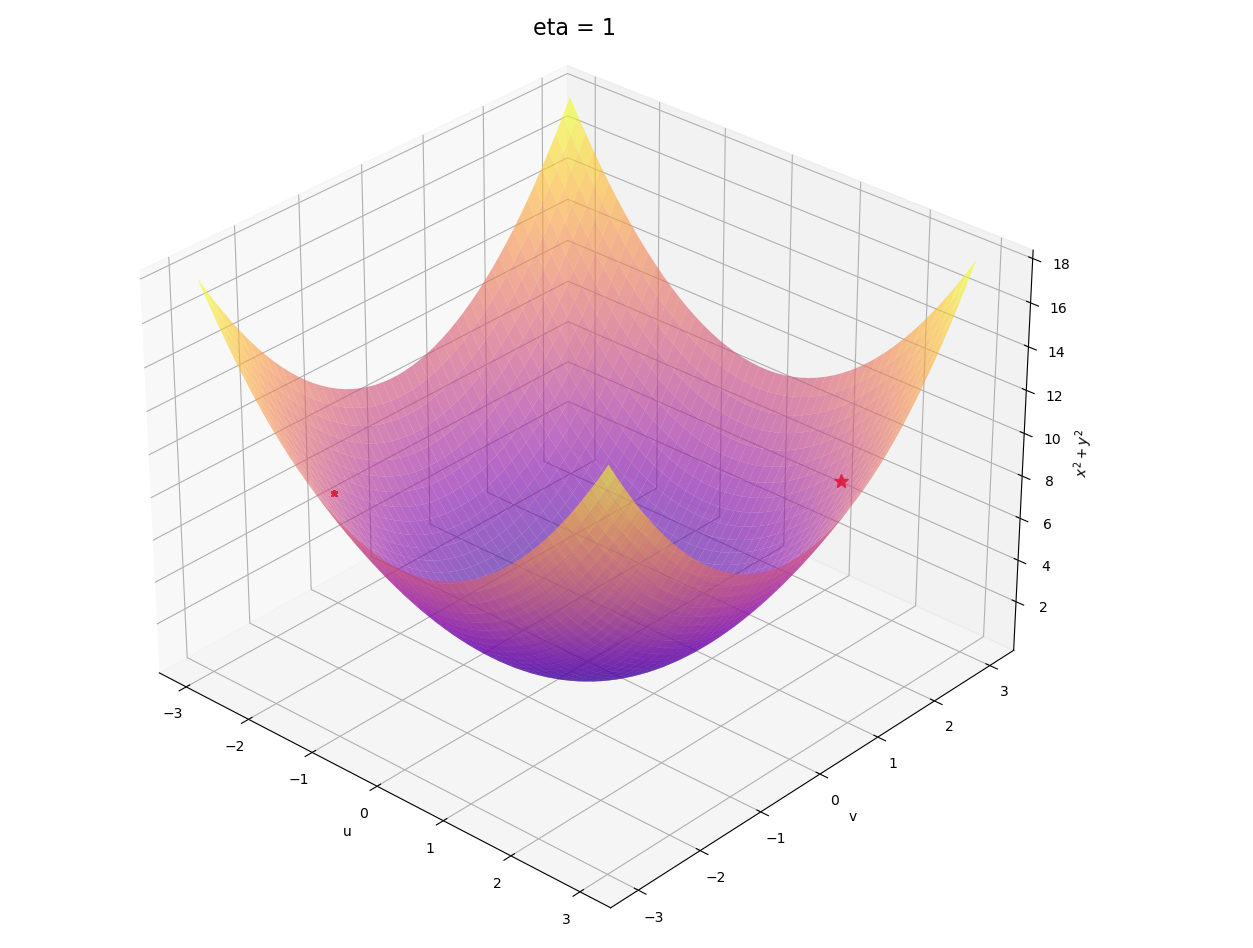
\includegraphics[width=0.75\textwidth]{eta1}
  \caption{$\eta = 1$}
  \label{fig:eta1}
\end{figure}
Como podemos ver en la imagen \ref{fig:eta1}, al tener un learning rate alto, los valores que vamos obteniendo en cada
paso no nos llevan a ningun lugar, pasa de $(2,2)$ hasta $(-2,-2)$ en cada iteracion.

Normalmente este valor esta entre el rango de $ 0.1 - 0.01$ y en nuestro caso lo dejaremos fijo.
\newpage
\begin{figure}
  \centering
   \subfloat[$x^2 + y^2$]{
    \label{f:f1}
     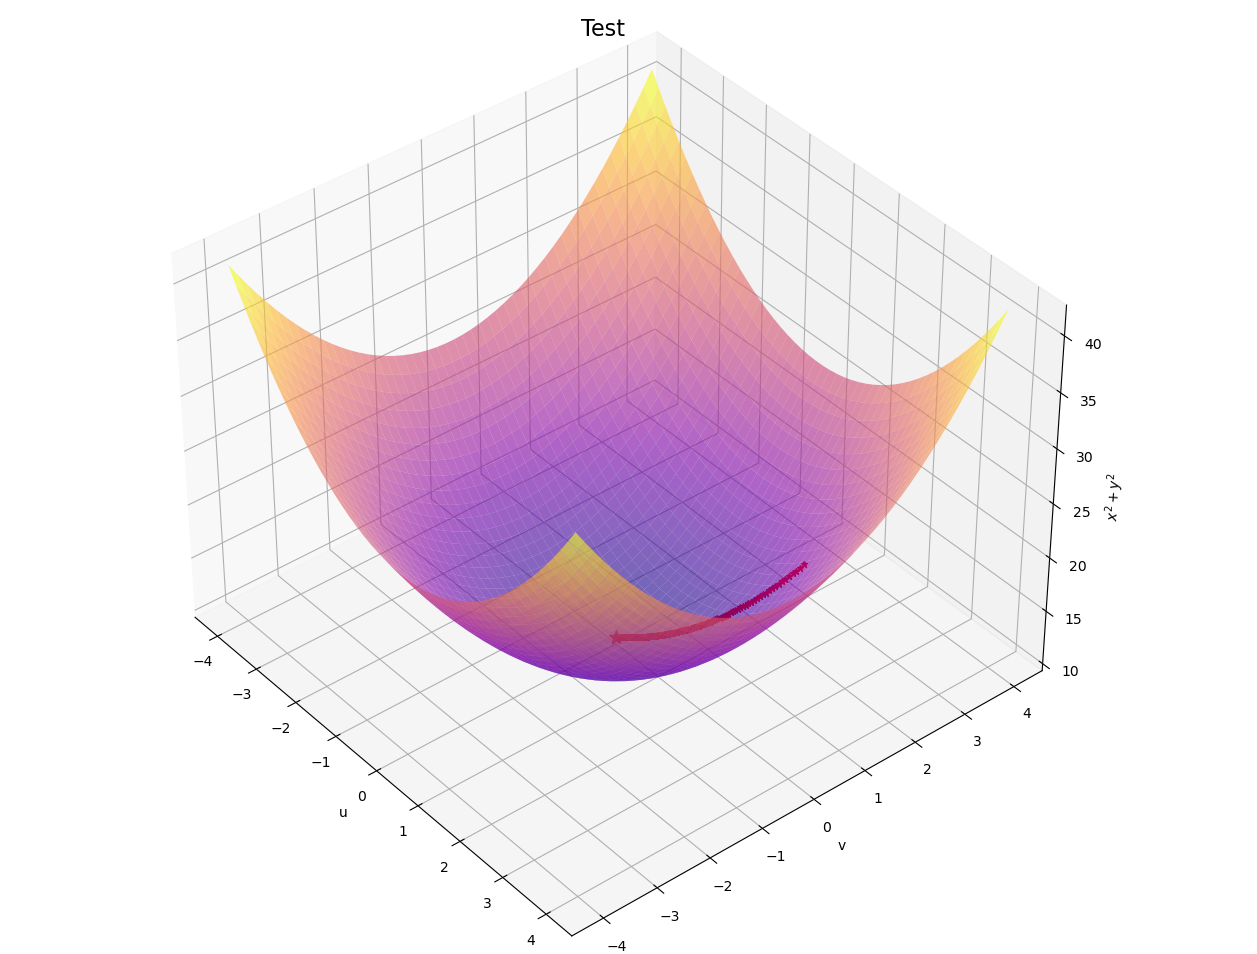
\includegraphics[width=0.5\textwidth]{Prueba1_gradiente}}
   \subfloat[$x^2 + y^2+x+10$]{
    \label{f:f2}
     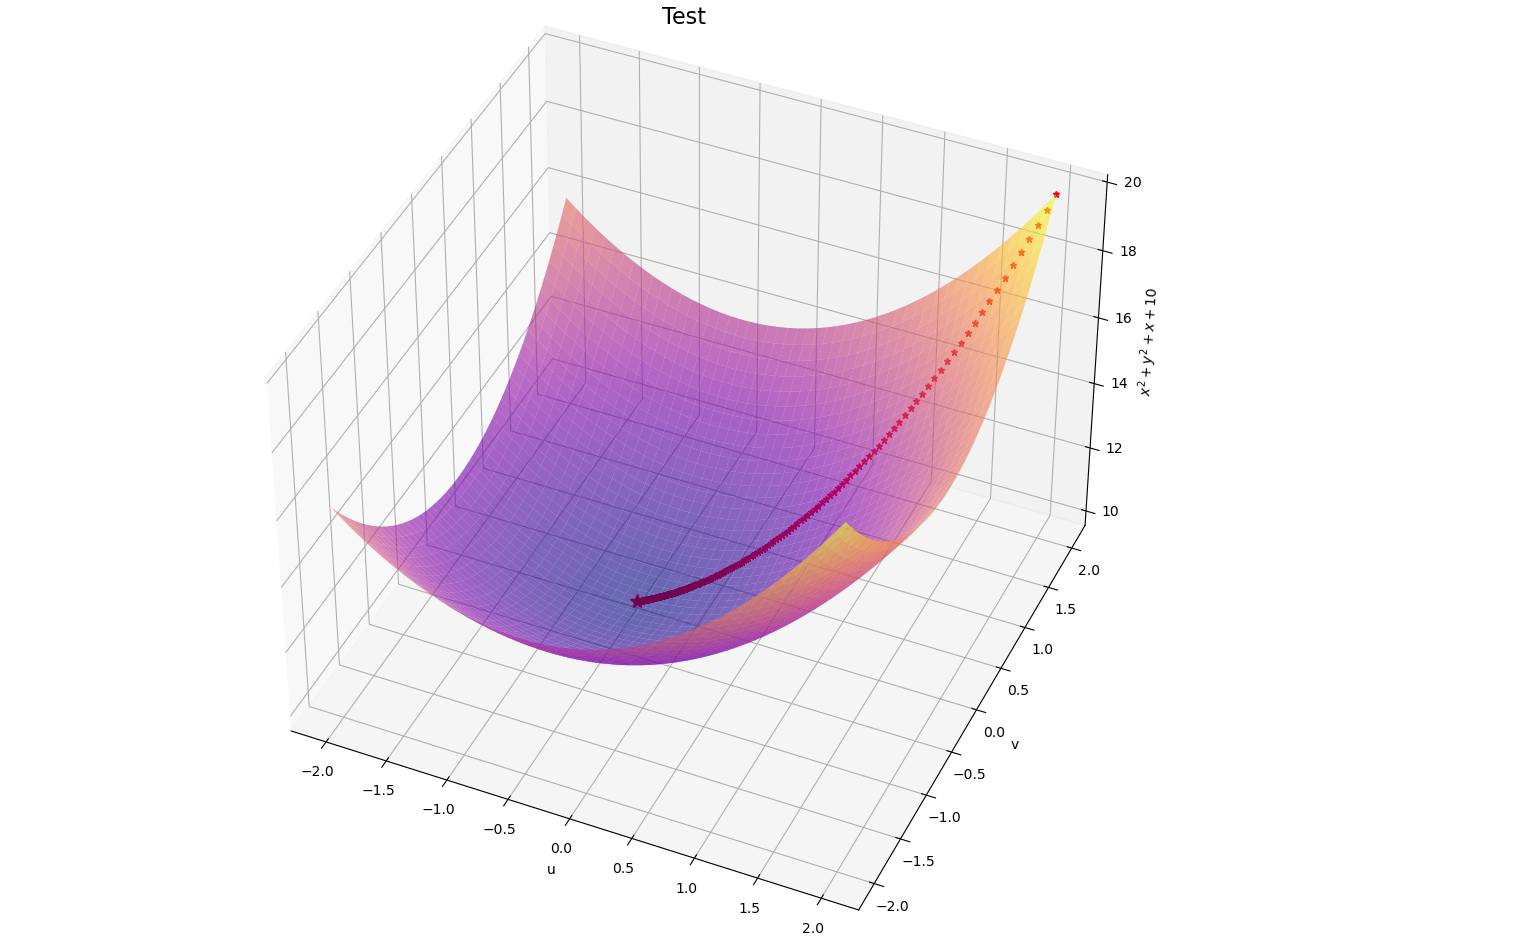
\includegraphics[width=0.6\textwidth]{Prueba2_gradiente}}
  \caption{Gradiente Descenciente}
  \label{f:Pruebas_gradiente}
 \end{figure}


 
 
\subsection{Implementacion del Algoritmo de Gradiente Descenciente}

La clave del gradiente sera $ \frac{\partial E_{in}(w)}{\partial w_j}$ , donde en este caso $E_{in}$ sera la funcion de error dentro de la muestra 
con respecto a $w$, w es un parámetro que minimiza la función. 

Entonces el algoritmo ira actualizando los coordenadas (w) de la siguiente forma\newline
$ w_j = w_j - \eta \frac{\partial E_{in}(w)}{\partial w_j}$ hasta un cierto numero de iteraciones o una precision dada.



\subsection{Ejercicio2}
\subsubsection{Calculo analitico de $E(u,v)$}
Considerando la funcion $E(u,v) =(u\cdot v\cdot e^{-u^2-v^2})^2$ sobre la cual tendremos que aplicar el Gradiente Descenciente para encontrar su minimo, necesitaremos calcular sus derivadas parciales.

\begin{itemize}
  \item $\displaystyle \frac{\partial E}{\partial u} = -2u(2u^2 -1)\cdot v^2 \cdot e^{-2(u^2+v^2)}$
  \item $\displaystyle \frac{\partial E}{\partial v} = -2u^2v (2v^2-1) \cdot e^{-2(u^2+v^2)}$
\end{itemize}

Ahora que tenemos las derivadas parciales podemos crear el gradiente de esta funcion, en nuestro caso un array cuyas dos componentes seran los pesos a minimizar
$np.array(\frac{\partial E}{\partial u}, \frac{\partial E}{\partial v})$
\newpage 
\subsubsection{Valor inferior a $10^{-8}$ en $E(u,v)$}
Como condiciones iniciales tenemos que comenzamos en $(u,v) = (0.5,-0.5)$ con un $\eta = 0.1$.

{
\begin{wrapfigure}{l}{0.5\textwidth}
  \centering
  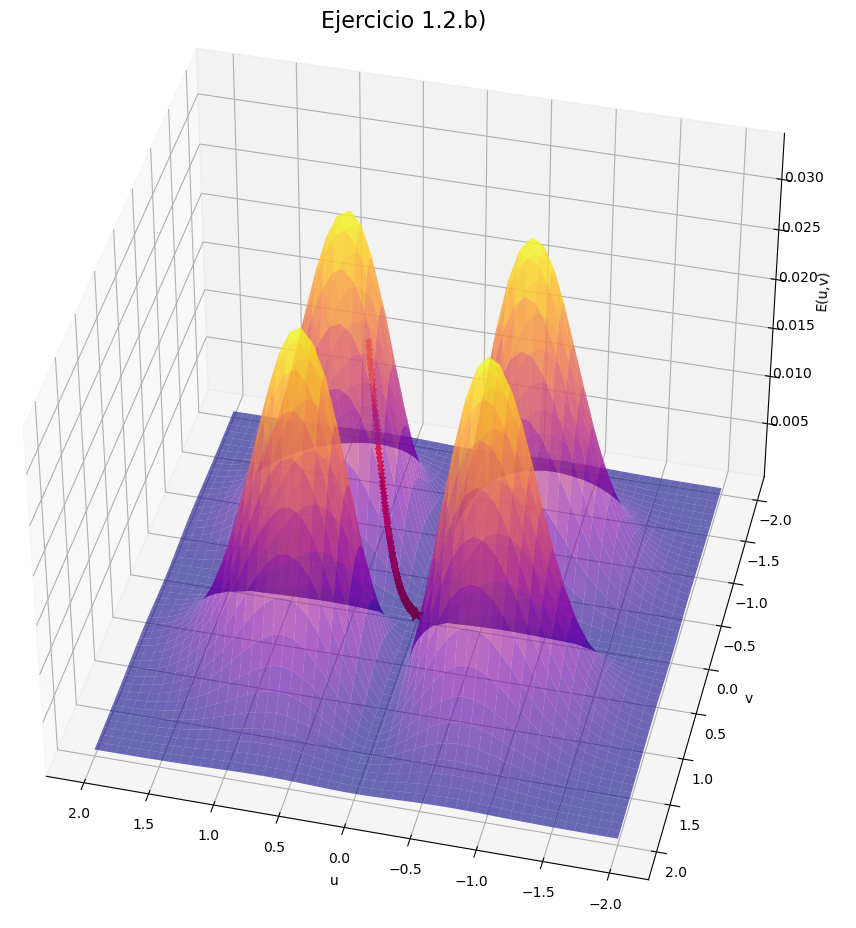
\includegraphics[width=0.8\linewidth]{min2E.png}
  \caption{Encontrando Minimo de $E(u,v)$}
\end{wrapfigure}

En mi caso partiendo de los datos iniciales, encuentro en 25117 Iteraciones un valor menor al error dado.

\par
\vspace{5mm}

\subsubsection{Coordenadas del minimo obtenido}
Tras haber haber obtenido un error menor a $10^{-8}$ las coordenadas obtenidas para el minimo son
\newline $( 0.010000842574554563 ,  -0.010000842574554563 )$
\vspace{30mm}

}
\subsection{Calculos para $f(x,y) = x^2+2y^2+2sin(2 \pi x)sin(\pi y)$}
%----------------------------------------------------------------------------------------

En esta grafica podemos ver lo lejos que se han quedado de encontrar
 el minimo ( los valores que alcanzan el 0 son que han encontrado el minimo ) con un numero maximo de 50 iteraciones para diferentes valores de  $\eta$ eje horizontal
 Como podemos ver para valores entre 0.05 y 0.07 y para valores superiores a 0.08 ya no es capaz de acercarse al minimo
\subsubsection{3a}
textooooooooo
 \begin{figure}[h]
  \centering
  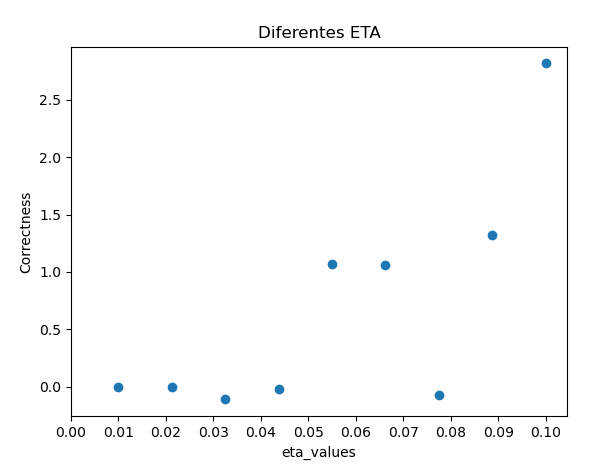
\includegraphics[width=0.5\textwidth]{correctness}
  \caption{Distancia al minimo}
  \label{fig:eta1}
\end{figure}
textooooooooo


\subsubsection{3b}
\begin{figure}[h]
  \centering
  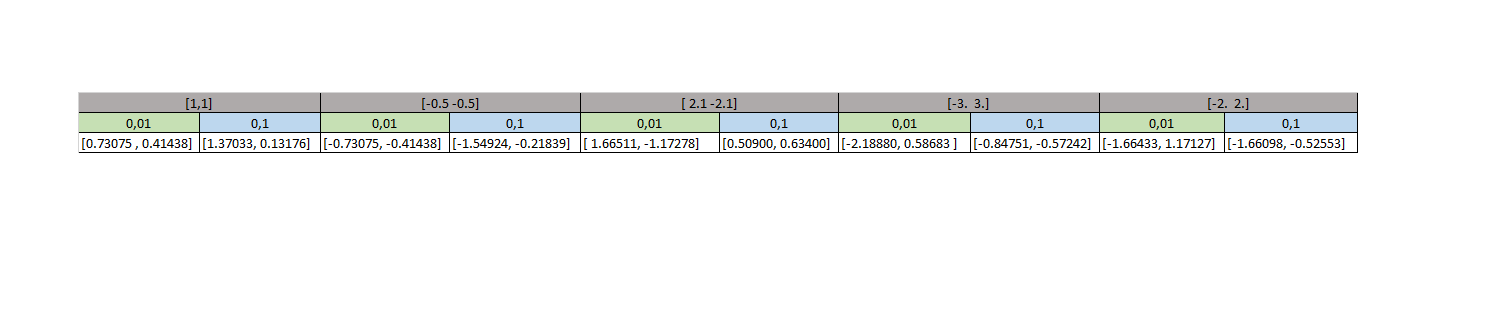
\includegraphics[width=0.90\textwidth]{Exvelpng}
  \caption{Resultados para $\eta = 0.01 $ y $ \eta = 0.1$}
  \label{fig:eta1}
\end{figure}
  
FALTA COMENTAR LAS DEPENDENCIAS SOBRE EL PUNTO INICIAL

\subsection{ conclusion sobre la verdadera dificultad de encontrar el mınimo
global de una funcion arbitraria}
%----------------------------------------------------------------------------------------
%	Cuestión 3
%----------------------------------------------------------------------------------------

\section{Regresion Lineal}




%------------------------------------------------

\bibliography{citas} %archivo citas.bib que contiene las entradas 
\bibliographystyle{plain} % hay varias formas de citar

\end{document}
